\documentclass[11pt,a4paper]{article}
\usepackage[margin=1in]{geometry}
\usepackage{tikz}
\usetikzlibrary{arrows,shapes,positioning,calc,decorations.pathmorphing}

\setlength{\emergencystretch}{2em}

\begin{document}

\begin{figure}[h]
\centering
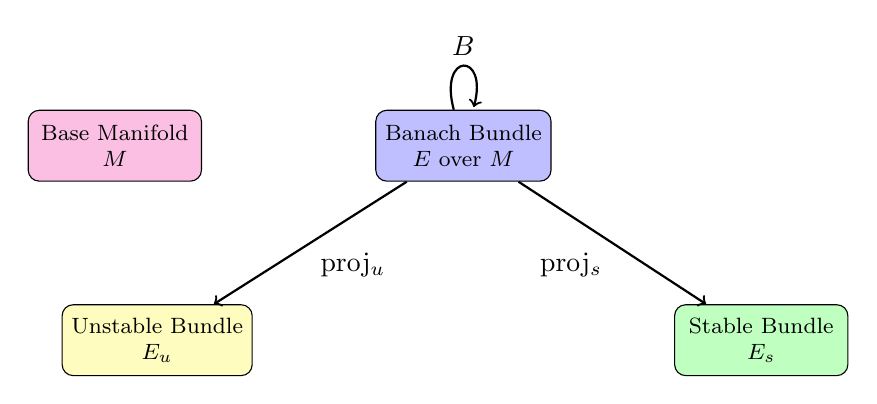
\begin{tikzpicture}[node distance=2.2cm, auto,
  nodest/.style={draw, rounded corners, minimum width=2.2cm, minimum height=0.9cm, align=center, font=\footnotesize}]
  \node[nodest, fill=magenta!25] (M) {Base Manifold\\$M$};
  \node[nodest, fill=blue!25, right=of M] (E) {Banach Bundle\\$E$ over $M$};
  \node[nodest, fill=green!25, below right=of E] (S) {Stable Bundle\\$E_s$};
  \node[nodest, fill=yellow!25, below left=of E] (U) {Unstable Bundle\\$E_u$};
  \draw[->, thick] (E) edge[loop above] node{$B$} (E);
  \draw[->, thick] (E) -- node[swap]{proj$_s$} (S);
  \draw[->, thick] (E) -- node{proj$_u$} (U);
\end{tikzpicture}
\caption{Graphical abstract: base manifold $M$, Banach bundle $E\to M$ with hyperbolic splitting $E=E_s\oplus E_u$, and the normal cocycle $B$ governing fibre deformation. Persistence of a normally hyperbolic invariant manifold reduces to solving $\mathcal A\zeta=\zeta\circ f-B\zeta=q$ under bunching $\bar{\mathfrak b}^\pm_{k,\alpha}<1$.}
\label{fig:graphical-abstract}
\end{figure}

\end{document}